%% EESP @ SC26 submission -- regular paper (8 pp, refs excluded).
%% Double-blind: author identity anonymized per CFP.
%% Template: IEEE conference proceedings (required by EESP CFP).
\documentclass[conference]{IEEEtran}
\IEEEoverridecommandlockouts

\usepackage{cite}
\usepackage{amsmath,amssymb}
\usepackage{graphicx}
\usepackage{booktabs}
\usepackage{multirow}
\usepackage{xcolor}
\usepackage{siunitx}
\usepackage{url}
\usepackage{xspace}
\usepackage[hidelinks]{hyperref}

\sisetup{group-separator={,}, group-minimum-digits=4}

% Allow line breaks in the long env-var name
\newcommand{\perfboost}{\texttt{\mbox{CUDA}\_\hspace{0pt}\mbox{DISABLE}\_\hspace{0pt}\mbox{PERF}\_\hspace{0pt}\mbox{BOOST}}\xspace}

\begin{document}

\title{The Model Parking Tax: A Configuration-Induced\\ Idle-Power Anomaly in GPU Serving}

\author{\IEEEauthorblockN{Anonymous Author(s)}
\IEEEauthorblockA{\textit{Submitted for double-blind review (EESP @ SC26)}}}

\maketitle

\begin{abstract}
Data centers face growing pressure to reduce energy use, yet inference GPUs spend much of their time idle---holding a model in memory to stay responsive while serving no requests. The power a GPU draws in this state is commonly treated as a fixed cost of readiness. We show that a large part of it---roughly a fifth to two-thirds, depending on the GPU---is not fixed at all, but an artifact of a driver default that is recoverable. Using 18~days of production telemetry from 14~H100 GPUs and controlled experiments on four GPU architectures (HBM3, HBM2e, GDDR6, and HBM3e), we find that idle power does not depend on the model a GPU holds---with a CUDA context resident, a GPU holding a ${\sim}77$\,GB model and one holding almost nothing draw the same---but on whether that context is present, which forces full clock speed even at zero utilization and adds 26--67\,W per GPU. Because this power is spent with no work to perform, it is an anomaly rather than a genuine cost of serving. We confirm the cause with a controlled experiment: holding the model fixed while setting a single driver flag (\perfboost) returns idle power toward its floor, recovering roughly 95--100\% of the overhead across architectures, with no measured latency penalty on the H100 and A100 and no throughput penalty in an H100 load test. At data-center scale, a mid-range scenario puts the recoverable overhead near \num{460}\,GWh per year (${\sim}180$\,kT CO$_2$). It is the most prominent of a broader class of \emph{configuration-induced idle-power anomalies}: cases where a configuration setting, not the workload, holds idle power above its floor.
\end{abstract}

\begin{IEEEkeywords}
GPU energy efficiency, idle power, DVFS, CUDA, LLM inference serving, sustainable computing, power measurement
\end{IEEEkeywords}

% ===========================================================================
\section{Introduction}
% ===========================================================================
The energy use of AI data centers is under intense scrutiny, and inference serving is a growing part of it. Much of this energy is spent while GPUs are idle. To avoid cold-start latency, serving systems keep models resident in GPU memory continuously, and utilization studies report that GPUs spend a large fraction of their time idle or underutilized: production fleets report roughly 35\% of capacity idle~\cite{flexera}, and execution-idle alone accounts for 19.7\% of in-execution time at cluster scale~\cite{lei-idle}. The 2024 U.S. Data Center Energy Usage Report places GPU idle power at ${\sim}20\%$ of thermal design power (TDP)~\cite{doe-report}. The idle power a GPU draws while holding a model but serving no request is generally treated as an unavoidable cost of readiness and is rarely examined.

This paper asks whether that cost is unavoidable, and finds that much of it is not. We decompose idle power and show that it does not come from the resident model: across four memory technologies, allocated memory has no measurable effect, and a fully loaded GPU idles at the same power as an almost-empty one. What determines idle power is a single configuration state---whether a CUDA context is present---which pins the GPU at full clock frequency even when it performs no work, adding 26--67\,W. This overhead is therefore an anomaly rather than an intrinsic cost of serving; because it is a configuration artifact, we show it can be removed outright.

Prior work touches the phenomenon but does not decompose it. Cold-start optimization is a rich literature~\cite{serverlessllm,nvidia-streamer,hydraserve,lambdascale}, but addresses the reload cost, not the idle power of resident models. Patel et al.~\cite{patel-cal23} observed that a CUDA context elevates A100 clocks at 0\% utilization, and Lei et al.~\cite{lei-idle} characterize how often execution-idle occurs at cluster scale. Neither measures the marginal idle cost \emph{per GB of allocated memory}, determines whether the cost is intrinsic to the resident model or an artifact of configuration, tests this across memory technologies, evaluates a mitigation, or places the phenomenon in a general class.

This paper makes four contributions:

\begin{enumerate}
\item \textbf{Idle power is not a cost of the resident model.} We decompose idle power and find it invariant to allocated VRAM (all four slopes $|\beta| < 0.02$\,W/GB; two one-sided tests bound the effect below the 0.1\,W/GB relevance threshold) across HBM3, HBM2e, GDDR6, and HBM3e (Blackwell) in both production telemetry and controlled experiments, consistent with the resident model not being its source (\S\ref{sec:model-doesnt-matter}).
\item \textbf{The overhead is a removable configuration artifact.} Idle power is a step function of CUDA-context presence. A controlled experiment that holds the model fixed and toggles a single driver flag recovers roughly 95--100\% of the overhead across four architectures, with no latency penalty measured on the H100 and A100 and no throughput penalty in an H100 load test, supporting the interpretation that the waste is a configuration artifact rather than a physical cost (\S\ref{sec:control-plane}).
\item \textbf{The behavior is consistent with a latency-oriented default.} It reduces first-request latency at the cost of continuous idle power; we quantify this trade-off and identify the regime---always-on serving---in which it is inappropriate (\S\ref{sec:default}).
\item \textbf{It generalizes to a class of configuration-induced idle-power anomalies.} We give a taxonomy and a principle for where large, recoverable idle waste occurs (\S\ref{sec:taxonomy}).
\end{enumerate}

Formally, idle power is
\begin{equation}
P_{\text{idle}}(C, V) = P_{\text{base}} + \Delta P_{\text{DVFS}} \cdot \mathbf{1}_{[C=1]} + \beta V,
\label{eq:model}
\end{equation}
with $\beta \approx 0$ and $\Delta P_{\text{DVFS}} \gg \beta V$ for any real model. The optimization priority is $\partial P/\partial C \gg \partial P/\partial V$: the context term dominates the model term.

% ===========================================================================
\section{Background: Why Memory Cannot Set Idle Power}
% ===========================================================================
\subsection{The DVFS anomaly}
NVIDIA datacenter GPUs support several power states via dynamic voltage and frequency scaling (DVFS). Without a CUDA context, streaming-multiprocessor (SM) clocks idle at 210--345\,MHz (architecture-dependent). The instant a CUDA context is created---by any runtime call---the SM clock jumps to maximum boost and \emph{remains there} at 0\% utilization~\cite{patel-cal23}. The expected behavior, $P \downarrow$ as utilization $U \to 0$, is replaced by $P = \text{const}$ whenever $C=1$. This converts a \emph{variable} cost into a \emph{fixed} one and, crucially, decouples idle power from both utilization and memory occupancy. It is the mechanism by which the cost stops being a property of the workload.

\subsection{Memory physics predicts $\beta \approx 0$}
That the model term is negligible is not merely an empirical result; it is predicted by DRAM physics. GPU memory power decomposes into background, refresh, and activation components~\cite{hbm-spec,micron-ddr}. Background power is constant whenever the memory clock runs. Refresh power is proportional to installed \emph{capacity}, not occupancy---refresh circuitry sweeps every row per JEDEC specification regardless of which rows hold valid data. Activation power (row open/close) is zero at idle. Hence $\partial P_{\text{mem}}/\partial\,\text{occupancy} \approx 0$: a model occupying more of an already-powered memory array adds essentially nothing. This holds for HBM3, HBM2e, and GDDR6 alike---all DRAM with mandatory refresh. Section~\ref{sec:model-doesnt-matter} tests this prediction directly, and it is why the invariance we report should be expected to generalize rather than being a quirk of one device.

\subsection{Was this known, and why does the flag exist?}
The boost-on-context behavior was documented by Patel et al.~\cite{patel-cal23} in 2023; the anomaly is not new. What is new is the mitigation and the framing. NVIDIA added the \perfboost environment variable in the 580 driver series (CUDA Toolkit 13.2, late 2025; publicly noted at driver 580.105.08, November 2025). As \S\ref{sec:default} argues, the behavior is consistent with a latency-optimizing default whose cost/benefit only recently tipped as always-on serving came to dominate GPU idle time; the flag lets operators opt out where a single global default---which cannot serve both latency-critical interactive and always-on serving workloads---no longer fits.

\subsection{Other related work}
Zeus~\cite{zeus} optimizes energy for \emph{active} training. Patel et al.~\cite{patel-asplos24} characterize LLM inference power \emph{phases} during active execution. Burtscher et al.~\cite{burtscher-power} show \texttt{nvidia-smi} samples power for only ${\sim}25\%$ of runtime---a caveat we address with long, low-variance steady-state windows (\S\ref{sec:method}). Lei et al.~\cite{lei-idle} quantify how often execution-idle occurs; we isolate what the idle cost is a property of, bound the memory term, and provide controlled evidence supporting a causal interpretation of the mechanism. Cold-start systems~\cite{serverlessllm,nvidia-streamer,hydraserve,lambdascale} optimize the reload cost but say nothing about the idle power of models that stay resident.

% ===========================================================================
\section{Methodology}
\label{sec:method}
% ===========================================================================
\paragraph{Phase~1: production telemetry}
We instrumented 14 H100 80GB SXM5 GPUs across 2~Kubernetes nodes on a production inference cluster. NVIDIA Data Center GPU Manager (DCGM) Exporter fed Prometheus at 30\,s intervals. We collected \num{336226} observations over 18~days; average utilization was 0.11\%, and filtering to strict 0\% utilization retained \num{335267} samples (99.7\%). VRAM allocations spanned 3\,MB to 77\,GB. The 18-day window was set by the production observation period, not chosen to hit a sample target: it spans multiple diurnal cycles and both weekday and weekend regimes, and captures the full VRAM range as models were deployed, scaled, and retired---so the reported memory-independence cannot be an artifact of a single deployment snapshot. With 30\,s sampling and thermal autocorrelation of 3--5\,min ($\tau \approx 6$--10 samples), the effective sample size is $N_{\text{eff}} \approx N_{\text{raw}}/(2\tau+1) \approx \num{16000}$--\num{26000}.

\paragraph{Phase~2: controlled dose-response}
Within-subject dose-response on the four GPUs in Table~\ref{tab:gpus}, each following one protocol: record bare-idle baseline (no context); create a persistent CUDA context; sequentially allocate increasing VRAM with \texttt{torch.empty}; at each level, stabilize 60\,s, then record \texttt{nvidia-smi} every 30\,s for 20\,min ($n=40$/phase); release; cool 30\,s. The three primary GPUs (H100, A100, L40S) use this full protocol; the B200 uses a shorter confirmation sweep (3-minute phases, $n=18$). We summarize each phase by its median power throughout, robust to the occasional single-sample DVFS transient (present in the H100 and Blackwell flag runs); on the dose-response phases the median and mean coincide within 1\,W, but transient-prone flag/idle phases can differ by a few watts, which is why we report medians. The within-subject design isolates VRAM as the sole manipulated variable and eliminates between-device confounders (silicon binning, cooling, power delivery). Within-phase standard deviation is $<1.5$\,W on the noisiest device (L40S) and $<0.17$\,W on the H100, giving standard error $<0.25$\,W. We apply the two one-sided tests (TOST) equivalence procedure~\cite{schuirmann-tost} with bound $\Delta = \pm 0.1$\,W/GB, so even a 64\,GB model contributes $<6.4$\,W---several-fold below the DVFS step (4--8$\times$, by architecture).

\paragraph{Phase~3: the control experiment}
We evaluate \perfboost on H100 80GB SXM (Hopper, driver 580.126.09) and A100 80GB SXM4 (Ampere, driver 580.126.16) under three conditions: baseline (context + \texttt{torch.empty} 16\,GB); flag on; and flag with vLLM~\cite{vllm} serving Qwen2.5-7B~\cite{qwen2} (fp16), measuring idle power between requests and latency (p50/p95/p99).

\paragraph{Phase~4: multi-GPU scaling}
On a single 4$\times$H100 80GB SXM node with NVLink (driver 580.126.09), 9~conditions using vLLM serving Qwen2.5-7B: bare idle, TP=2/4, DP=2, TP=2$\times$DP=2, each with and without the flag. Per condition we measured warm latency ($n=50$), the DVFS decay curve (5\,min at 1\,s), steady-state idle power ($n=40$, 20\,min), and the cold-start ramp (60\,s idle soak, then 1 cold + 4 recovery requests).

\begin{table}[t]
\caption{Phase~2 GPU configurations. The first three GPUs used 30\,s sampling and 20-minute phases ($n=40$); the B200 used a shorter confirmation sweep (3-minute phases, $n=18$).}
\label{tab:gpus}
\centering
\small
\begin{tabular}{llrr}
\toprule
\textbf{GPU} & \textbf{Memory} & \textbf{TDP} & \textbf{VRAM swept} \\
\midrule
H100 80GB SXM & HBM3 & 700\,W & 0--64\,GB \\
A100 80GB PCIe & HBM2e & 300\,W & 0--72\,GB \\
L40S 48GB & GDDR6 & 350\,W & 0--40\,GB \\
B200 180GB SXM & HBM3e & 1000\,W & 0--32\,GB \\
\bottomrule
\end{tabular}
\end{table}

% ===========================================================================
\section{Idle Power Is Not a Cost of the Resident Model}
\label{sec:model-doesnt-matter}
% ===========================================================================
We test whether idle power is an intrinsic cost of the resident model---whether it scales with the memory the model occupies. If it did, idle power would increase with VRAM occupancy. It does not, on any architecture or memory technology tested, nor in production. This rules out the resident model as the source of the idle cost and points to a configuration cause, which \S\ref{sec:control-plane} identifies and shows to be removable.

\subsection{Production telemetry: two discrete power states}
Phase~1 telemetry is bimodal: 7~GPUs at bare idle (345\,MHz, $74.7 \pm 7.9$\,W) and 7~at CUDA-active idle (1980\,MHz, $145.5 \pm 11.2$\,W). The context effect is $+70.9$\,W (Cohen's $d = 7.3$, $p < 10^{-300}$). Within the CUDA-active GPUs---which span 3.2--77.1\,GB of resident model state---regression against VRAM gives slope $0.013$\,W/GB ($R^2 = 0.001$, $p = 0.95$): no detectable relationship between how much model a GPU holds and how much idle power it draws. Node-level variation from silicon binning and cooling (${\sim}23$\,W) already dwarfs any memory effect. The two power states are separated by context presence, not by model size.

\subsection{Controlled dose-response across architectures}
Table~\ref{tab:cross} and Fig.~\ref{fig:hero} isolate the effect. On all four GPUs, creating a context triggers a discrete DVFS step of $+26.3$\,W (A100) to $+67.2$\,W (L40S); then \emph{sweeping VRAM from 0 to 32--72\,GB changes power by less than 1\,W}. The context accounts for $>99\%$ of the parking tax on every device. Computed on the per-phase means, the 95\% CIs for the VRAM slope are $[-0.006,+0.003]$ (H100), $[-0.002,-0.001]$ (A100), and $[-0.026,+0.022]$ (L40S)\,W/GB. TOST rejects $|\beta| \ge 0.1$\,W/GB on every device ($p_{\text{TOST}} < 0.05$): under our tested protocol we do not merely fail to find a memory effect but bound it several-fold (4--8$\times$) below the DVFS step. Because the sweep is sequential on one device per architecture, the effective observations are the per-phase means rather than the individual correlated samples, and the design cannot fully separate a small VRAM term from slow time or thermal drift---the A100 and B200 slopes are two such confounds. The invariance holds across four memory technologies (HBM3, HBM2e, GDDR6, HBM3e) spanning bandwidths from 864\,GB/s to 3.35\,TB/s---exactly as the refresh-dominated physics of \S{II-B} predicts. Figure~\ref{fig:decomp} makes the decomposition visual: the model's contribution is invisible at scale.

\begin{table}[t]
\caption{Cross-architecture parking tax. $\beta$ is the VRAM regression slope across CUDA-active phases; all GPUs at 0\% utilization. The context term dominates; the model term is statistically indistinguishable from zero.}
\label{tab:cross}
\centering
\scriptsize
\setlength{\tabcolsep}{3.5pt}
\begin{tabular}{lrrrr}
\toprule
 & \textbf{H100} & \textbf{A100} & \textbf{L40S} & \textbf{B200} \\
 & \textbf{(HBM3)} & \textbf{(HBM2e)} & \textbf{(GDDR6)} & \textbf{(HBM3e)} \\
\midrule
Bare idle (W) & 71.8 & 53.7 & 35.6 & 181.7 \\
SM clk, bare (MHz) & 345 & 210 & 210 & 120 \\
CUDA-ctx power (W) & 121.7 & 80.0 & 102.7 & 233.6 \\
SM clk, ctx (MHz) & 1980 & 1410 & 2520 & 1965 \\
\midrule
\textbf{Context overhead (W)} & \textbf{+49.9} & \textbf{+26.3} & \textbf{+67.2} & \textbf{+51.9} \\
Context (\% of TDP) & 7.1\% & 8.8\% & 19.2\% & 5.2\% \\
\midrule
Max VRAM tested (GB) & 64 & 72 & 40 & 32 \\
$\beta$ (W/GB) & $-$0.002 & $-$0.001$^\dagger$ & $-$0.002 & $+$0.019$^\dagger$ \\
$p_{\text{TOST}}$ ($|\beta|<0.1$) & $10^{-9}$ & $<0.001$ & $<0.05$ & $<0.01$ \\
\midrule
\textbf{Context \% of tax} & \textbf{$>$99\%} & \textbf{$>$99\%} & \textbf{$>$99\%} & \textbf{$>$99\%} \\
\bottomrule
\end{tabular}
\par\vspace{2pt}
\parbox{\columnwidth}{\footnotesize $^\dagger$Slope significant but a temporal/thermal artifact of the sequential sweep (A100 negative, B200 positive); $<$1\,W total, far below the 0.1\,W/GB bound. All power values are per-phase medians, robust to occasional single-sample DVFS transients.}
\end{table}

\begin{figure*}[t]
\centering
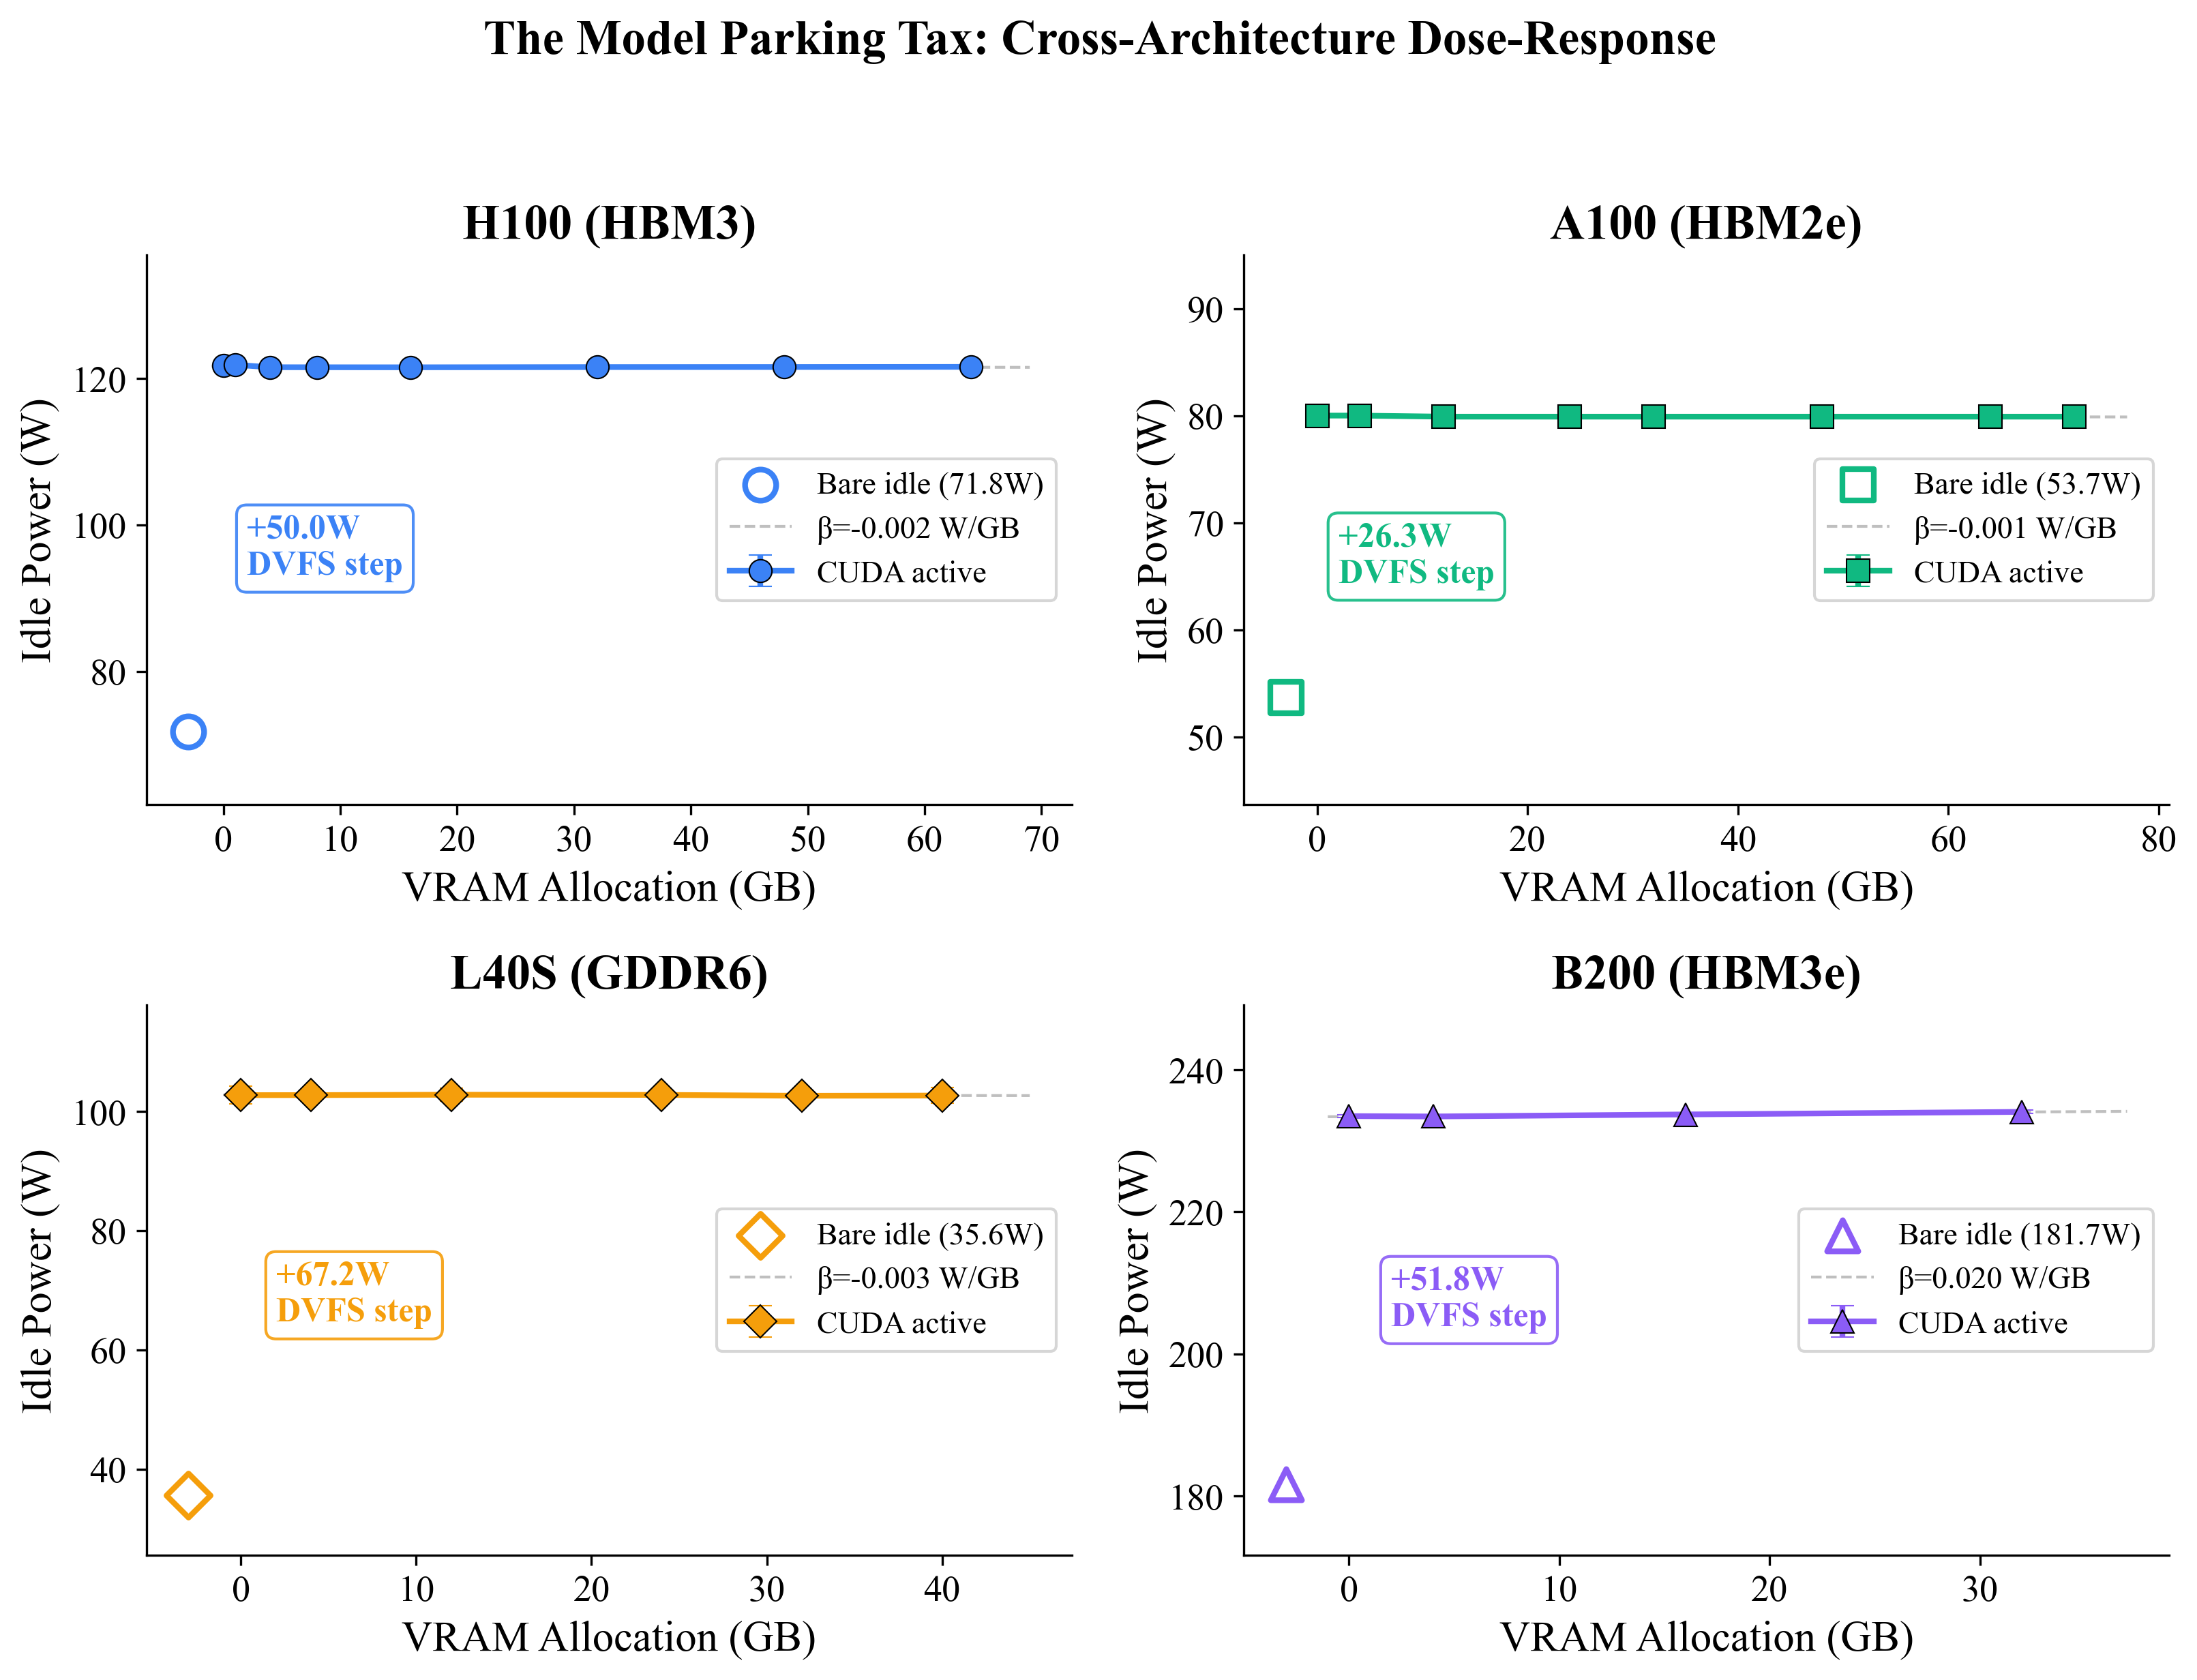
\includegraphics[width=0.86\textwidth]{cross_architecture_dose_response.png}
\caption{The model parking tax across four GPU architectures. Large markers (``bare''): bare-idle power with no CUDA context. Connected lines: CUDA-active phases with increasing VRAM. The discrete DVFS step dominates on every device; all four dose-response curves are flat across HBM3, HBM2e, GDDR6, and HBM3e (Blackwell). More model does not mean more idle power.}
\label{fig:hero}
\end{figure*}

\paragraph{The A100 negative slope}
\label{sec:a100}
On the A100, $\beta = -0.001$\,W/GB ($p = 0.002$): statistically significant but \emph{negative}, totaling $-0.09$\,W across 72\,GB and coinciding with a $0.7^\circ$C HBM temperature drift over the sequential run. More memory cannot reduce power; this is a temporal confound, not physics. It is a cautionary case: even a $p<0.05$ ``effect'' here is 300$\times$ smaller than the DVFS step and points the wrong way---which is why we report equivalence bounds rather than a null-hypothesis test.

\begin{figure}[t]
\centering
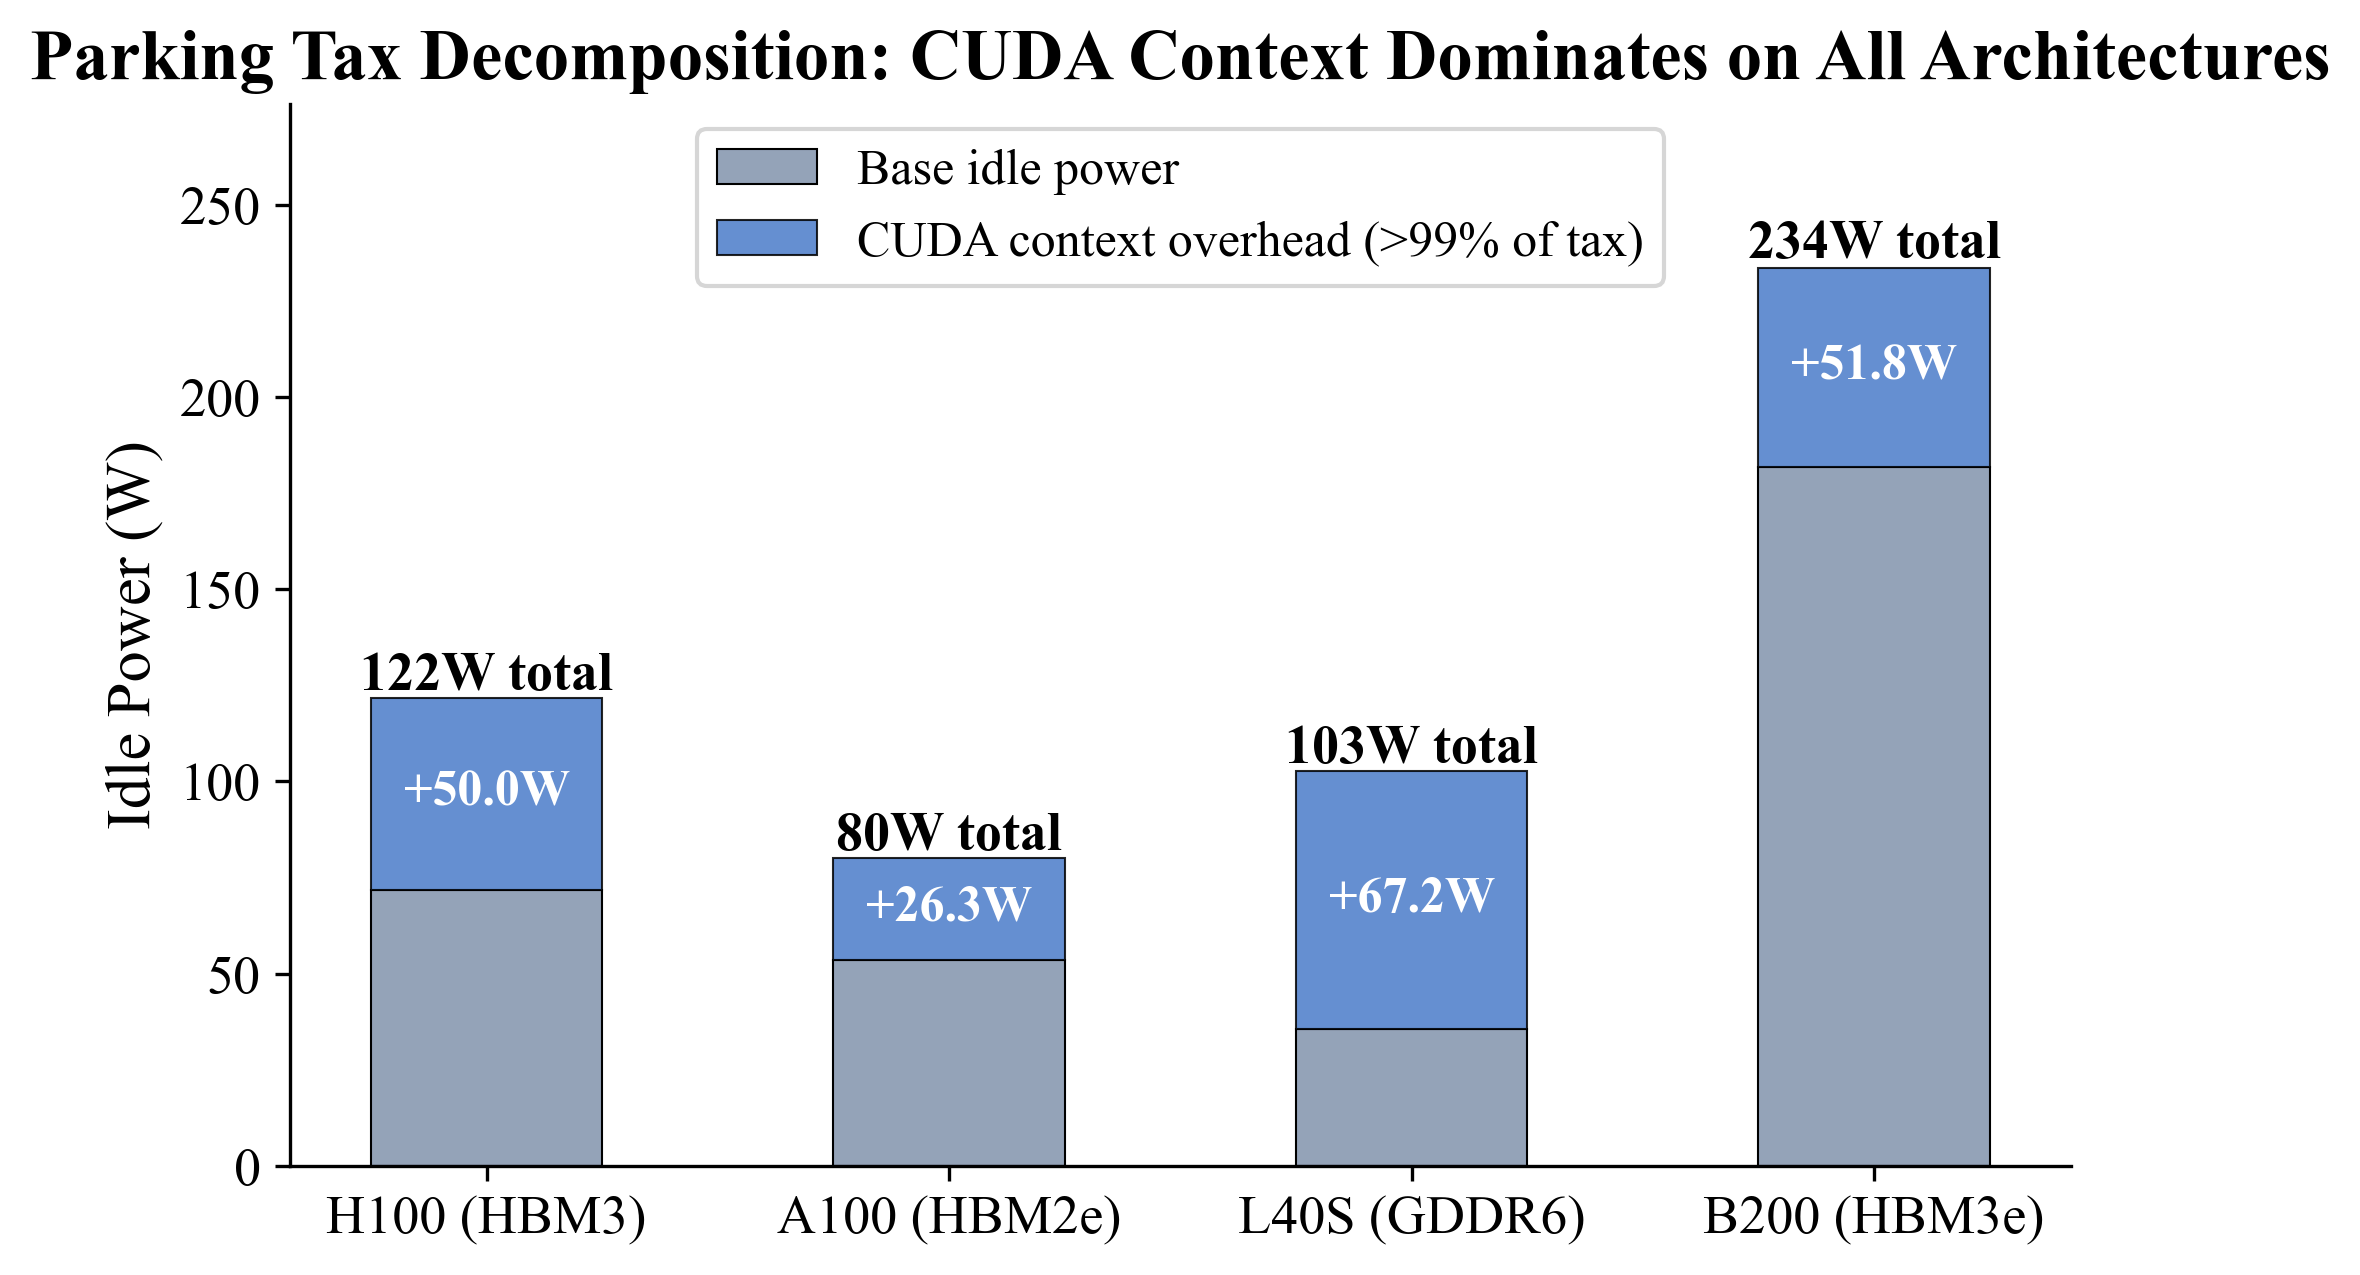
\includegraphics[width=\columnwidth]{parking_tax_decomposition.png}
\caption{Parking-tax decomposition. Gray: base idle power. Color: CUDA-context overhead ($>$99\% of the tax on every architecture). The VRAM term is too small to render.}
\label{fig:decomp}
\end{figure}

\paragraph{Blackwell (HBM3e)}
On the B200 (Blackwell, HBM3e) we ran the same dose-response over four VRAM levels (3-minute phases, $n=18$). Creating a context raises idle power from 182\,W (120\,MHz) to 234\,W (1965\,MHz)---a 52\,W tax at 0\% utilization---and power stays flat within 1\,W across 0--32\,GB, matching the other three architectures. The boosting default is present on this current-generation part.

\subsection{Validation with real model weights}
A skeptic might expect real model weights---with their CUDA kernels, cuDNN handles, and tensors---to behave differently from \texttt{torch.empty}. They do not (Table~\ref{tab:validation}). On the H100, Qwen2.5-7B idles within 0.03\,W of a 16\,GB empty allocation, despite the real model's CUDA kernels, cuDNN handles, and tensors. A real 7B model loaded on the L40S idles at 105.85\,W, in line with the context-active idle level measured for that architecture in Phase~2 (absolute idle power varies across instances, tracking the inter-node spread of Phase~1). Whether a GPU holds a real 7B model or an equivalent block of empty memory, the idle cost is set by whether a context is resident, not by the model.

\begin{table}[t]
\caption{Real-model validation on the H100. A real Qwen2.5-7B (fp16) idles within 0.03\,W of a 16\,GB \texttt{torch.empty} allocation holding the same CUDA context; the delta is within measurement noise.}
\label{tab:validation}
\centering
\small
\begin{tabular}{@{}llrrr@{}}
\toprule
\textbf{GPU} & \textbf{Allocation} & \textbf{VRAM (GB)} & \textbf{Idle (W)} & $\Delta$ \\
\midrule
\multirow{2}{*}{H100} & \texttt{torch.empty} 16\,GB & 16.0 & 121.51 & --- \\
 & Qwen2.5-7B & 14.9 & 121.48 & $-$0.03 \\
\bottomrule
\end{tabular}
\end{table}

% ===========================================================================
\section{Idle Power Is Determined by the CUDA Context}
\label{sec:control-plane}
% ===========================================================================
Section~II identifies the CUDA context, acting through the DVFS boost, as the mechanism. We now test this with a controlled experiment rather than relying on correlation.

\subsection{The control experiment}
This is a controlled test that supports a causal interpretation. If idle power were determined by the model, then changing a driver setting while holding the model, its weights, and its VRAM footprint fixed would leave idle power unchanged. Instead, setting \perfboost to \texttt{1} holds the H100's SM clock at the bare-idle 345\,MHz even with an active context and 16\,GB resident, and idle power falls from 128.1\,W to 73.2\,W (median; two transient DVFS samples inflate the raw mean to 75.9\,W), indistinguishable from bare idle (73.3\,W). On the A100 SXM4 the flag recovers 96\% of the 11.1\,W overhead. Because the model is held fixed and only the driver flag changes, the 55\,W reduction is attributable to the CUDA context rather than to model size (Table~\ref{tab:flag}, Fig.~\ref{fig:flagpower}).

Beyond its practical value as a one-line mitigation, the flag serves here as the experimental manipulation that isolates the CUDA context as the cause of the overhead.

\begin{table}[t]
\caption{The control experiment: hold the model fixed, toggle one bit. Idle: $n=40$, 20-min phases. Latency: $n=50$ warm requests (128-tok prompt/completion). Cold: first request after a 60\,s idle soak.}
\label{tab:flag}
\centering
\small
\begin{tabular}{@{}lrrrr@{}}
\toprule
 & \multicolumn{2}{c}{\textbf{H100 SXM}} & \multicolumn{2}{c}{\textbf{A100 SXM4}} \\
\cmidrule(lr){2-3}\cmidrule(lr){4-5}
 & \textbf{Base} & \textbf{Flag} & \textbf{Base} & \textbf{Flag} \\
\midrule
Idle power (W) & 128.1 & 73.2 & 75.1 & 64.5 \\
SM clock (MHz) & 1980 & 345 & 1155 & 210 \\
Tax recovered & --- & $>$99\% & --- & 96\% \\
\midrule
vLLM idle (W) & 128.6 & 73.1 & 73.9 & 64.3 \\
Warm latency (ms) & 533.4 & 533.3 & 910.0 & 910.0 \\
Cold req.\,1 (ms) & 546 & 683 & 921 & 1{,}130 \\
Ramp penalty (ms) & $+$10 & $+$147 & $+$11 & $+$220 \\
\bottomrule
\end{tabular}
\end{table}

\begin{figure*}[t]
\centering
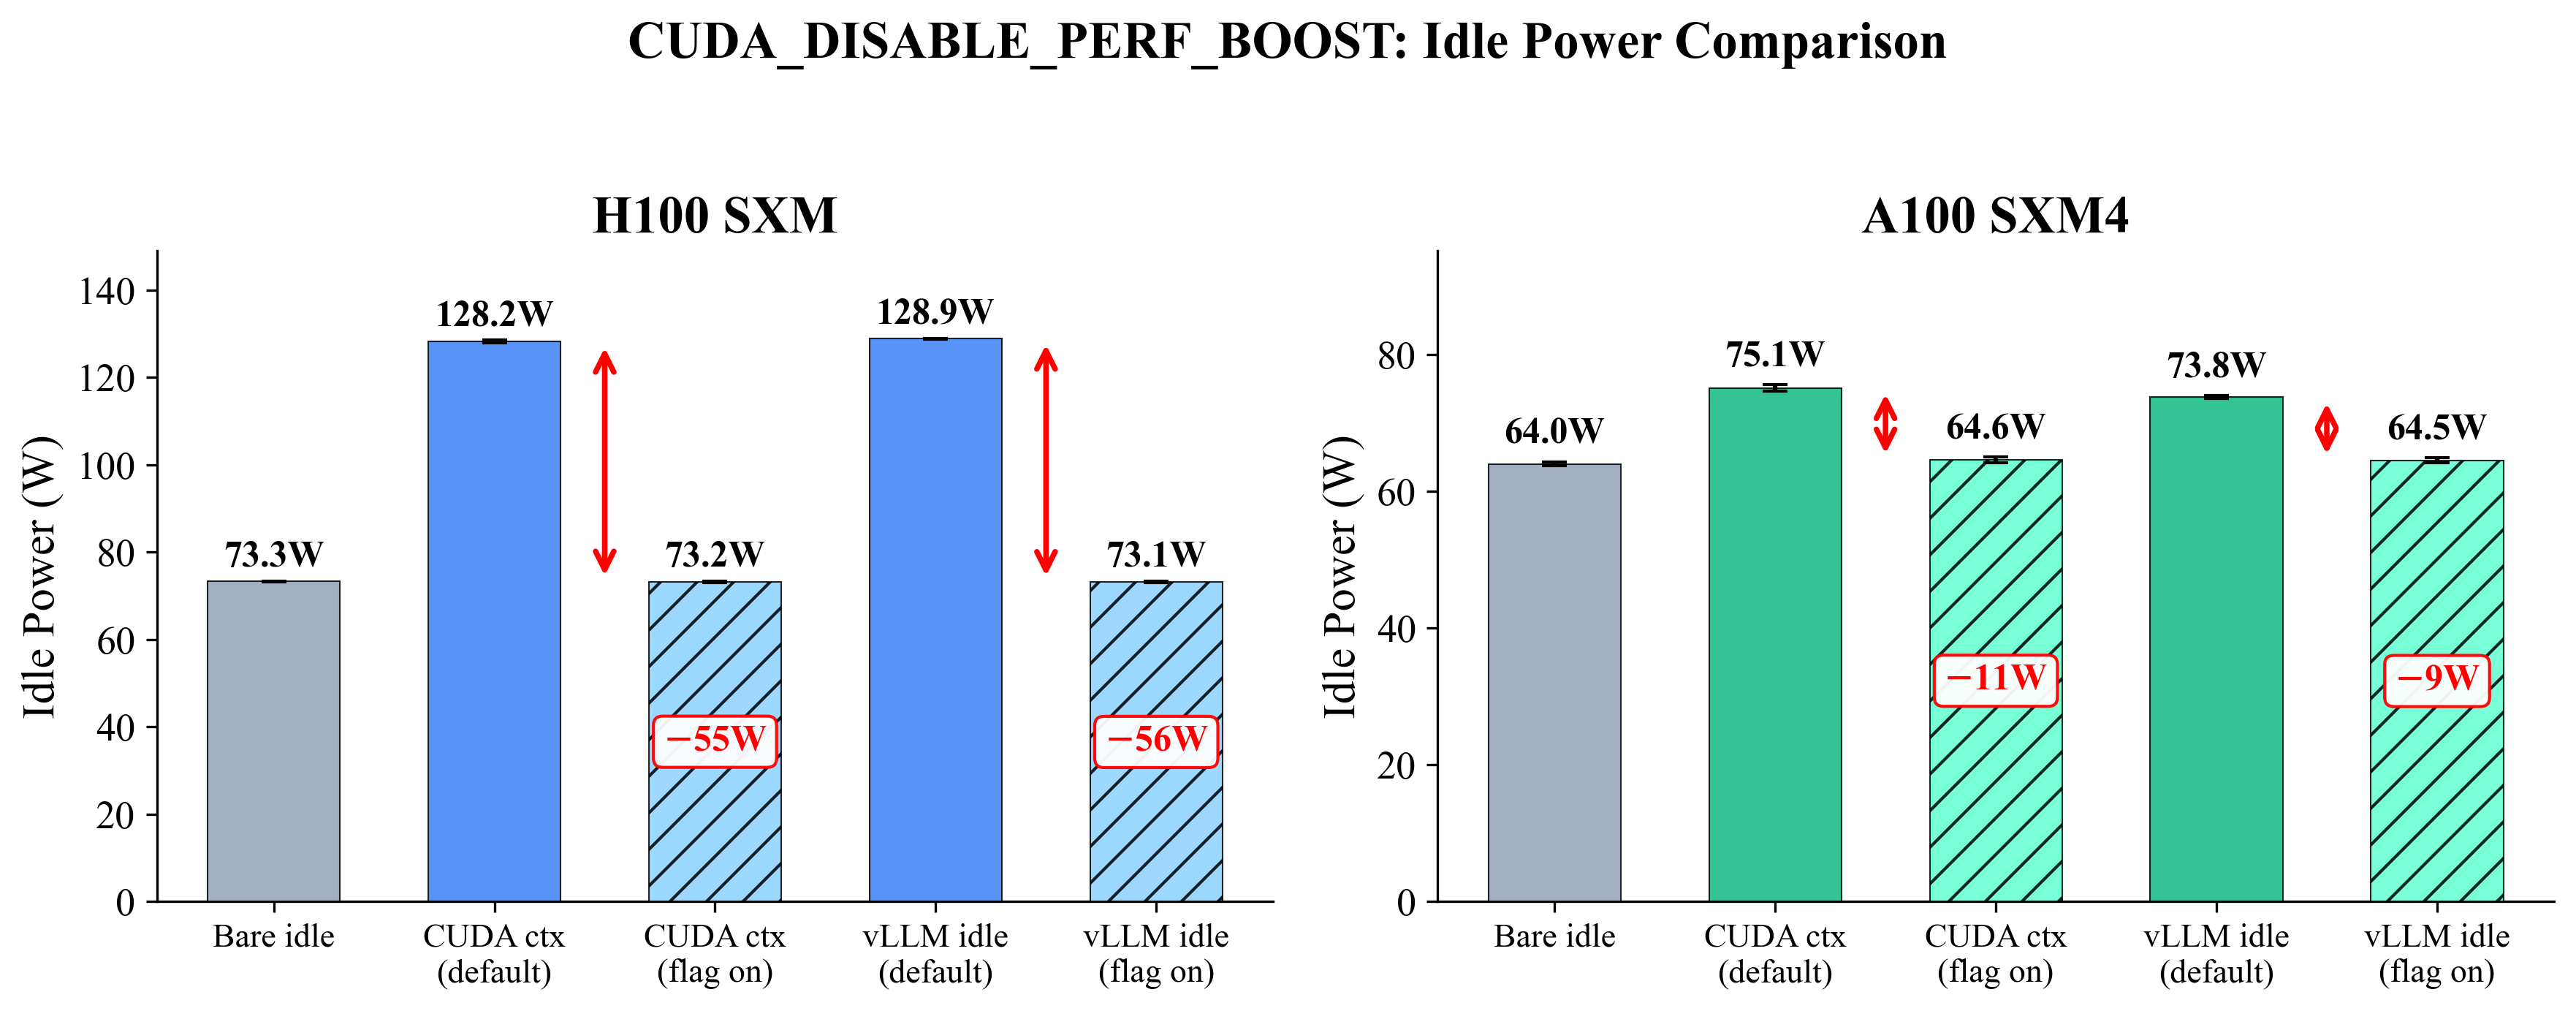
\includegraphics[width=0.86\textwidth]{perf_boost_power_comparison.png}
\caption{The control experiment, visualized. Hatched bars: flag enabled. On both H100 and A100 the flag collapses idle-with-context power to bare-idle levels---whether the context comes from \texttt{torch.empty} or a full vLLM stack with ${\sim}72$\,GB of reserved VRAM. The model is identical across each pair; only the driver flag differs.}
\label{fig:flagpower}
\end{figure*}

\paragraph{The mitigation holds across architectures}
Beyond the H100 and A100 (Table~\ref{tab:flag}), we measured the flag's idle-power effect on the L40S and B200 with an idle-only protocol. On the L40S---the highest-tax device---context-active idle falls from 102\,W (2520\,MHz) to 36.8\,W (210\,MHz), the bare-idle floor: essentially the full tax recovered. On the Blackwell B200 the flag returns idle power to the same floor: with the flag set, median context-active idle falls from 234\,W to 182\,W (the bare-idle floor), and the SM clock dropped to 120\,MHz in 71 of 72 context-active samples, with one transient boost during the 4\,GB phase. Across all four architectures the flag recovers roughly 95--100\% of the context overhead.

\paragraph{No steady-state cost}
Through vLLM serving Qwen2.5-7B, steady-state warm latency is similar to baseline in this retest on both architectures (Table~\ref{tab:flag}; a single 50-request run per condition, not repeated runs); vLLM's decode-phase CUDA graphs function correctly under the flag. The flag suppresses only the \emph{idle} boost; under load, clocks still rise to full frequency. A high-concurrency throughput benchmark on the H100 supports this (Qwen2.5-7B, 512 requests at concurrency~64): in a single run, aggregate decode throughput was 9287\,tok/s at baseline and 9355\,tok/s with the flag (a 0.7\% difference); repeated trials would be needed to characterize run-to-run variance. In both conditions the GPU held the same 1980\,MHz SM clock---its full boost frequency---and drew ${\sim}534$\,W, so the flag does not cap active clocks. The only cost is a one-time DVFS ramp on the first request after idle ($+147$\,ms H100, $+220$\,ms A100), gone by request~2; a keep-alive probe could mask it at the cost of the idle power it is meant to save---a trade-off we do not measure.

\subsection{The cost scales with configuration, not workload}
If the cost is per-context, it should multiply with the number of contexts and be indifferent to what those contexts compute. Table~\ref{tab:multigpu} and Fig.~\ref{fig:multigpu} confirm both. Across tensor, data, and mixed parallelism on a 4$\times$H100 node, the per-GPU tax is ${\sim}52$\,W---matching the single-GPU H100 figure---and the communication pattern is irrelevant: NCCL all-reduce (TP), independent contexts (DP), and mixed all produce the same per-GPU overhead. The tax scales linearly,
\begin{equation}
P_{\text{park}}(N) = N \cdot \Delta P_{\text{DVFS}} \approx N \times 52\,\text{W (H100)},
\label{eq:linear}
\end{equation}
so a 4-GPU node wastes ${\sim}216$\,W idle and an 8-GPU node ${\sim}430$\,W---determined by how many contexts are resident, not by the model or the interconnect. Every flag-on condition drops per-GPU idle to within 0.6\,W of bare idle. Warm latency is similar to baseline throughout (one run per condition).

The cold-start ramp does \emph{not} compound with $N$: it is $+145$--176\,ms across all configurations, matching the single-GPU ${\sim}150$\,ms. Under TP, the first kernel launch triggers NCCL collectives that act as implicit barriers, so all $N$ GPUs ramp in parallel and user-facing latency is bounded by the slowest single ramp; under DP each replica ramps independently. Without the flag, clocks stay locked at 1980\,MHz for the full 5-minute decay window---the governor never self-corrects; with the flag, clocks fall to 345\,MHz within 2\,s of the last request and power settles to bare idle in $<4$\,s. The flag is set once at process start; no runtime toggling is needed.

\begin{table}[t]
\caption{The tax scales with the number of contexts, not the workload (4$\times$H100 SXM, Qwen2.5-7B fp16). Tax: per-GPU overhead vs.\ bare idle (71.7\,W). Cold penalty: first request after 60\,s idle minus recovery mean.}
\label{tab:multigpu}
\centering
\small
\begin{tabular}{@{}lrrrr@{}}
\toprule
\textbf{Condition} & \textbf{Per-GPU} & \textbf{Tax/} & \textbf{Warm} & \textbf{Cold} \\
 & \textbf{(W)} & \textbf{GPU} & \textbf{(ms)} & \textbf{pen.\,(ms)} \\
\midrule
Bare idle & 71.7 & --- & --- & --- \\
\midrule
TP=2 baseline & 124.9 & $+$53.2 & 340.3 & $+$5.4 \\
TP=2 flag on & 71.8 & $+$0.0 & 352.9 & $+$175.5 \\
TP=4 baseline & 125.6 & $+$53.9 & 237.7 & $+$13.8 \\
TP=4 flag on & 71.8 & $+$0.1 & 250.6 & $+$156.5 \\
DP=2 baseline & 123.0 & $+$51.3 & 531.4 & $+$5.0 \\
DP=2 flag on & 71.5 & $-$0.2 & 520.7 & $+$153.4 \\
TP2$\times$DP2 base & 125.8 & $+$54.1 & 352.9 & $+$7.2 \\
TP2$\times$DP2 flag & 72.3 & $+$0.6 & 353.1 & $+$144.9 \\
\bottomrule
\end{tabular}
\end{table}

\begin{figure}[t]
\centering
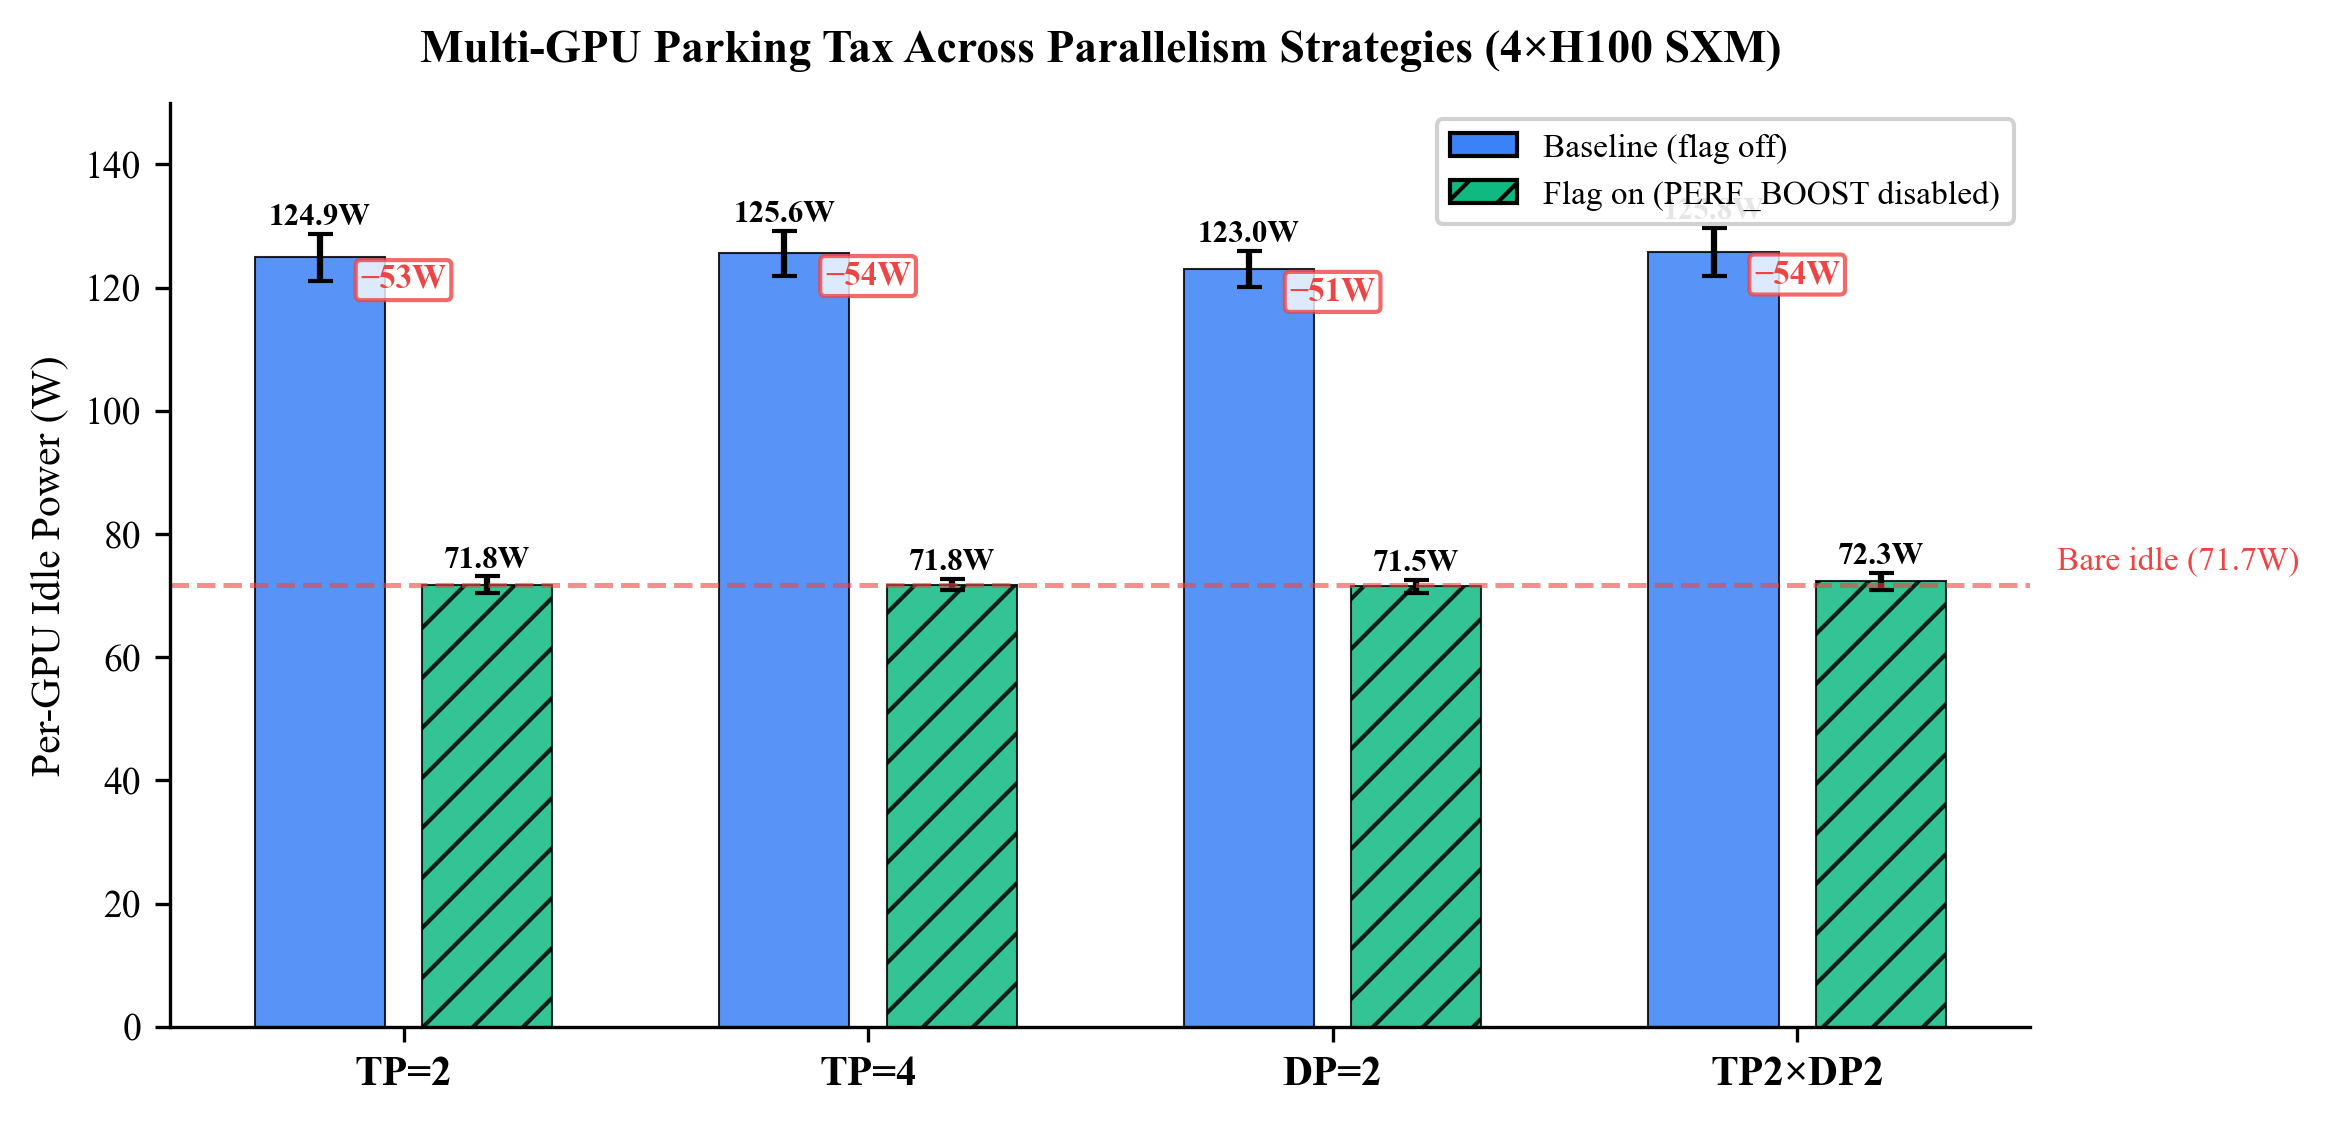
\includegraphics[width=\columnwidth]{multi_gpu_parking_tax.png}
\caption{Per-GPU idle power across parallelism strategies on a 4$\times$H100 SXM node. Baseline: ${\sim}125$\,W/GPU ($+53$\,W tax). Flag on (hatched): ${\sim}72$\,W/GPU (bare idle). The tax is consistent across TP, DP, and mixed configurations---the communication pattern does not matter, only the number of resident contexts.}
\label{fig:multigpu}
\end{figure}

% ===========================================================================
\section{The Boost Default and Its Operating Regime}
\label{sec:default}
% ===========================================================================
The boosting behavior is consistent with a default that favors first-request latency. Determining the regime in which it is inappropriate requires weighing the latency it avoids against the energy it costs.

Pre-ramping clocks the instant a context is created eliminates the DVFS ramp on the first kernel, which benefits \emph{sporadic interactive} workloads where any request may follow a long idle gap and tail latency is contractual. This behavior trades continuous idle power for reduced first-request latency, and the trade-off can be quantified. Keeping boost active during an idle gap of duration $t_{\text{gap}}$ costs
\begin{equation}
E_{\text{default}} = \Delta P_{\text{DVFS}} \cdot t_{\text{gap}}
\label{eq:default-cost}
\end{equation}
to save a one-time ramp of ${\sim}0.15$\,s on at most one request. On an H100 ($\Delta P_{\text{DVFS}} \approx 50$\,W), a $t_{\text{gap}}$ of just 1\,s spends ${\sim}50$\,J to shave 150\,ms off a single request; a 60\,s gap spends ${\sim}0.83$\,Wh. The default pays energy continuously to hedge a bounded, one-time latency cost.

The decision rule follows. Let $g$ be the fraction of requests that arrive after an idle gap long enough to have dropped clocks, and let an SLO tolerate added tail latency $\tau_{\text{SLO}}$. The default is justified only when the ramp would violate the SLO \emph{and} cold arrivals are common ($r > \tau_{\text{SLO}}$ and $g$ large). For always-on serving---the segment that, by Phase~1 and Lei et al.~\cite{lei-idle}, dominates GPU idle time---requests are batched and warm, $g$ is small, and the ${\sim}150$\,ms ramp (gone by request~2, removable with a keep-alive) rarely threatens a realistic SLO. In this regime the default is the wrong energy policy, and the flag should be the default. For sub-second-SLO interactive endpoints with mostly-cold arrivals, the vendor default remains defensible. A single global default cannot be correct for both regimes; the flag exists because the appropriate choice is per-deployment. The parking tax is the cost incurred when a latency-oriented default is applied to always-on serving workloads.

% ===========================================================================
\section{A Class of Configuration-Induced Idle-Power Anomalies}
\label{sec:taxonomy}
% ===========================================================================
The parking tax is one instance of a more general phenomenon: a \emph{configuration-induced idle-power anomaly}, in which idle power sits above the hardware floor $P_{\text{base}}$ because a persistent configuration setting holds a hardware domain above its idle state, independent of workload. Generalizing Eq.~\ref{eq:model},
\begin{equation}
P_{\text{idle}} = P_{\text{base}} + \sum_k \Delta_k \cdot \mathbf{1}[\text{config}_k=\text{on}],
\label{eq:general}
\end{equation}
where each term $\Delta_k$ is contributed by a persistent configuration setting rather than by workload, and the parking tax is the term $\Delta_{\text{DVFS}}\!\cdot\!\mathbf{1}[C=1]$. We measured this term directly; the value of the generalization is a principle, derived from mechanism, for which configuration settings can contribute a large $\Delta_k$ and which cannot.

The principle turns on which hardware domain a setting holds above its idle state. Settings that pin a \emph{clock} domain raise idle power by tens of watts, because dynamic power scales steeply with frequency and voltage; the CUDA-context DVFS boost measured here is the instance we study. Settings that touch only \emph{link or controller} state leave idle power near its floor: PCIe link power management, memory-clock locking, and persistence mode~\cite{nvidia-smi} act on domains that already idle at low power, and a power cap limits peak draw rather than idle clocks. Memory occupancy belongs to this second category---its idle contribution is dominated by occupancy-independent DRAM refresh---which is why the model term vanishes in Eq.~\ref{eq:model}. Because the parking-tax term is per-context, partitioning a GPU into multiple CUDA contexts through MIG or MPS multiplies it, as \S\ref{sec:consequences} discusses. For a new accelerator, the large idle-energy savings are found by identifying clock domains that a configuration setting holds above their idle frequency.

% ===========================================================================
\section{Implications for Serving Operators}
\label{sec:consequences}
% ===========================================================================
The preceding results have several direct implications for how inference is deployed.

\paragraph{Keep-warm decisions should not use model size}
Eviction and keep-warm policies that prioritize by footprint---evict the largest model first, keep small models warm because they are ``cheap''---optimize a variable that does not move idle power. The correct key is the number of resident contexts and the request arrival rate, not the model. A small model kept warm costs the same parking tax as a large one.

\paragraph{Eviction fallback when the flag is unavailable}
On older drivers or non-NVIDIA hardware, the fallback is to evict and cold-start. The energy break-even is $T^{*} = P_{\text{load}}\,t_{\text{load}}/P_{\text{park}}$: on an H100 ($P_{\text{park}}=49.9$\,W), standard PyTorch loading of a 70B model (${\sim}300$\,W, 45\,s) gives $T^{*}\approx 4.5$\,min, and fast loaders shrink it to tens of seconds. A $T^{*}$-based policy saves 8--23\% energy over always-on in trace simulation, and most on bursty traffic. Note that $T^{*}$ depends on load power and duration, not on model size.

\paragraph{The flag is preferable to eviction unless VRAM must be reclaimed}
Where the flag is available, keeping the model warm with the flag dominates eviction: it removes the tax while avoiding the full cold-start cost, paying only the ${\sim}150$\,ms ramp. Eviction earns its keep only when the freed VRAM has a waiting tenant. The reclaim question---not model size---is the deciding variable between ``flag and keep warm'' and ``evict.''

\paragraph{Context consolidation and configuration auditing}
Because the tax is per-context (Eq.~\ref{eq:general}), MPS~\cite{nvidia-mps}, which routes multiple clients through a single context, is itself an idle-energy optimization---the tax is paid once and amortized. MIG~\cite{nvidia-mig}, which gives each instance its own context, is predicted to pay the tax \emph{per instance}, so its isolation carries an energy cost proportional to partition count; a $k$-slice GPU could carry up to $k$ DVFS terms. We did not measure multi-tenant configurations---this is the most important untested prediction of Eq.~\ref{eq:general}, and it is directly falsifiable with the protocol used here. More broadly, operators should audit fleets for Class-A anomalies as a first-class energy lever, alongside the kernel- and scheduler-level optimizations that receive most attention.

% ===========================================================================
\section{Industry-Scale Impact}
% ===========================================================================
Let $N$ be total datacenter GPUs, $\rho$ average utilization, and $T_{\text{year}}=8760$\,h:
\begin{equation}
E_{\text{park}} = N(1-\rho)\cdot \bar{P}_{\text{park}} \cdot T_{\text{year}}.
\label{eq:industry}
\end{equation}
We present this as a scenario, not a measurement. Taking ${\sim}3.76$M datacenter GPUs (2023 annual shipments~\cite{nvidia-shipments}, a lower bound on the installed base), indicative $\rho = 0.65$ (35\% idle~\cite{flexera}), and a fleet-weighted $\bar{P}_{\text{park}} = 40$\,W applied only to context-resident idle GPUs, the base estimate is ${\sim}460$\,GWh/year (${\sim}180$\,kT CO$_2$ at U.S. grid average). Varying each input over its plausible range (fleet 2.0--6.0M, $\rho$ 0.50--0.80, $\bar{P}_{\text{park}}$ 26.3--67.2\,W) yields a wide 92--\num{1766}\,GWh/year band. The dominant uncertainty is fleet composition and duty cycle---not the per-GPU tax, which we measure directly. Even the lower bound exceeds a small city's annual electricity use.

% ===========================================================================
\section{Discussion and Limitations}
% ===========================================================================
\paragraph{Newer architectures and vendor power profiles}
We observe the same result on all four microarchitectures---Hopper, Ampere, Ada Lovelace, and Blackwell. On the B200 the context tax is 52\,W (182$\to$234\,W), flat across VRAM (HBM3e), and the flag returns median idle power to the 120\,MHz bare floor (234$\to$182\,W; 71 of 72 context-active samples at the floor, one transient boost). The mechanism is a driver-level DVFS governor, not an architecture-specific circuit, consistent with the invariance across all four generations. NVIDIA has introduced datacenter workload power profiles (including a Max-Q profile) on Blackwell B200~\cite{nvidia-power-profiles}, a coarse-grained, opt-in mechanism that selects hardware settings per workload class (training, inference, or HPC). By NVIDIA's description these profiles optimize \emph{active}-workload efficiency---redistributing power during computation---rather than idle power, and none targets the context-boost overhead measured here. The parking tax is therefore orthogonal to and unaddressed by current power profiles: a fine-grained, idle-side configuration artifact rather than a coarse-grained, active-side control. The \perfboost flag itself remains opt-in and off by default through the current driver series.

\paragraph{Adoption is an incentive problem}
The flag has been available since November 2025 but is exposed by neither vLLM~\cite{vllm}, SGLang, nor TensorRT-LLM, and its interaction with CUDA graphs was not publicly validated before this work. The market splits incentives: the engineers configuring inference engines are usually not the ones paying the power bill, and cloud tenants on flat hourly rates have no visibility into idle power. Native support in serving frameworks would let the operators who bear the cost act at fleet scale---the same principal-agent gap that lets a stale default persist.

\paragraph{Limitations}
We test one device per architecture in the main study, complemented by 14~H100s in Phase~1; the Blackwell runs use shorter phases ($n=18$) than the other three ($n=40$). Multi-GPU experiments cover a single 4$\times$H100 NVLink node; pipeline parallelism, 8-GPU nodes, NVSwitch fabrics, and multi-node deployments are untested, though the per-context mechanism suggests the per-GPU result is interconnect-independent. We measure one model size (Qwen2.5-7B); larger models may load differently, though memory-independence is tested to 72\,GB. The taxonomy rows other than the DVFS term are analytical, derived from documented mechanism, not measured here.

% ===========================================================================
\section{Conclusion}
% ===========================================================================
The cost of keeping a model warm in GPU memory is not a property of the model. Across four architectures spanning HBM3, HBM2e, GDDR6, and HBM3e (Blackwell), in production and in controlled experiment, idle power is invariant to model size (all four slopes $|\beta|<0.02$\,W/GB, bounded well below the 0.1\,W/GB relevance threshold by two one-sided tests) and is instead a step function of a single control-plane state---whether a CUDA context is resident, which forces a 26--67\,W DVFS boost. A controlled experiment that holds the model fixed and toggles a single driver flag recovers roughly 95--100\% of the overhead, attributing it to the CUDA context rather than to model size. The behavior is consistent with a latency-oriented default that is inappropriate for the always-on serving workloads that now dominate idle time, and it is the dominant member of a broader class of configuration-induced idle-power anomalies, for which we give a taxonomy and a detection principle. These results imply that size-based keep-warm and eviction heuristics optimize a variable that does not affect idle power; the relevant parameters are the number of resident contexts and the request arrival rate. At fleet scale, a mid-range scenario puts the recoverable overhead near \num{460}\,GWh/year, addressable through a one-line configuration change.

% ===========================================================================
\begin{thebibliography}{20}

\bibitem{patel-cal23}
T.~Patel, D.~Tiwari, et al., ``Towards improved power management in cloud GPUs,'' \emph{IEEE Computer Architecture Letters (CAL)}, 2023.

\bibitem{doe-report}
A.~Shehabi et al., ``2024 United States Data Center Energy Usage Report,'' Lawrence Berkeley National Laboratory, Dec.\ 2024.

\bibitem{serverlessllm}
Y.~Fu et al., ``ServerlessLLM: Low-latency serverless inference for large language models,'' in \emph{OSDI}, 2024.

\bibitem{nvidia-streamer}
NVIDIA, ``Reducing cold start latency for LLM inference with NVIDIA Run:ai Model Streamer,'' Tech.\ report, Oct.\ 2025.

\bibitem{hydraserve}
``HydraServe: Minimizing cold starts for serverless LLM serving,'' \emph{arXiv:2502.15524}, 2025.

\bibitem{lambdascale}
``$\lambda$Scale: Enabling fast scaling for serverless large language model inference,'' \emph{arXiv:2502.09922}, 2025.

\bibitem{lei-idle}
Y.~Lei, J.~Fernandez, V.~Kypriotis, D.~Skarlatos, E.~Strubell, J.~Sherry, and D.~Vosler, ``The energy cost of execution-idle in GPU clusters,'' \emph{arXiv:2604.04745}, Apr.\ 2026.

\bibitem{zeus}
J.~You et al., ``Zeus: Understanding and optimizing GPU energy consumption of DNN training,'' in \emph{NSDI}, 2023.

\bibitem{patel-asplos24}
T.~Patel et al., ``Characterizing power management opportunities for LLMs in the cloud,'' in \emph{ASPLOS}, 2024.

\bibitem{burtscher-power}
M.~Burtscher et al., ``Part-time power measurements: nvidia-smi's lack of attention,'' \emph{arXiv:2312.02741}, 2023.

\bibitem{flexera}
Flexera, ``2025 State of the Cloud Report,'' 2025.

\bibitem{nvidia-shipments}
Semiconductor industry estimates of NVIDIA datacenter GPU shipments, 2023.

\bibitem{hbm-spec}
JEDEC, ``HBM3 High Bandwidth Memory Specification (JESD238),'' 2022.

\bibitem{micron-ddr}
Micron Technology, ``TN-46-09: DRAM Power Calculations,'' Tech.\ Note, 2023.

\bibitem{schuirmann-tost}
D.~J.~Schuirmann, ``A comparison of the two one-sided tests procedure and the power approach for assessing the equivalence of average bioavailability,'' \emph{J.\ Pharmacokinetics and Biopharmaceutics}, 15(6):657--680, 1987.

\bibitem{nvidia-smi}
NVIDIA, ``NVIDIA System Management Interface (nvidia-smi) documentation,'' NVIDIA Documentation, 2024.

\bibitem{nvidia-mig}
NVIDIA, ``Multi-Instance GPU User Guide,'' NVIDIA Documentation, 2024.

\bibitem{nvidia-mps}
NVIDIA, ``Multi-Process Service,'' NVIDIA Documentation, 2024.

\bibitem{qwen2}
Qwen Team, ``Qwen2.5 Technical Report,'' \emph{arXiv:2412.15115}, 2024.

\bibitem{vllm}
W.~Kwon et al., ``Efficient memory management for large language model serving with PagedAttention,'' in \emph{SOSP}, 2023.

\bibitem{nvidia-power-profiles}
NVIDIA, ``Optimize data center efficiency for AI and HPC workloads with power profiles,'' NVIDIA Technical Blog, 2025.

\end{thebibliography}

\end{document}
